%+----------------------------------------------------------------------------+
%| SLIDES: 36 months presentation
%| Contents: 11 Techincal Slides + Status of Phd Milestones 
%|					 (extimated duration 3 minutes per slide )
%| Author: Antonio miti
%| Place: Leuven, September 2019
%+----------------------------------------------------------------------------+


%- HandOut Flag -----------------------------------------------------------------------------------------
\newif\ifHandout
	\Handouttrue  %uncomment for the printable version


%- D0cum3nt ----------------------------------------------------------------------------------------------
\ifHandout
	\documentclass[handout,10pt]{beamer}   
	\setbeameroption{show notes} %print notes    
\else
	\documentclass[10pt]{beamer}
\fi


%- Packages ----------------------------------------------------------------------------------------------
\usepackage{verbatim}
\usepackage{appendixnumberbeamer}
\usepackage[mode=buildnew,subpreambles=true]{standalone}
\usepackage{amsmath, amssymb}
\usepackage{tikz}
\usetikzlibrary{decorations.pathmorphing}
\usepackage{tikz-cd}
\usepackage{graphicx, animate}
\usepackage{hyperref}
\usepackage[english]{babel}
\usepackage{csquotes}
\usepackage{wasysym}
%\usepackage{enumitem} %option in itemize
\usepackage{xcolor}




%--Beamer Style-----------------------------------------------------------------------------------------------
\usetheme{toninus}

%- T1tle P4g3 -------------------------------------------------------------------------------------------
\title{Homotopy moment maps in Multisymplectic Geometry} 
\subtitle{\href{https://set.kuleuven.be/phd/sap/dualjoint/oral}{36th month presentation}}
\author[AMM]{\href{https://dmf.unicatt.it/miti/}{Antonio Michele Miti}}
\institute[UCSC and KU Leuven]{
  \begin{tabular}[h]{ccc}
      Università Cattolica del Sacro Cuore & $\qquad$ & KU Leuven \\
      Brescia, Italy & & Leuven, Belgium \\
      \href{https://dipartimenti.unicatt.it/dmf-home?rdeLocaleAttr=it}{
\includegraphics[width=3.5cm]{Logos/UnicattBS-logo}} & & 
      \href{https://wis.kuleuven.be/english}{
\includegraphics[width=4cm]{Logos/KULeuven_logo}}
  \end{tabular}      
}
\date[KULeuven_19] % (optional, should be abbreviation of conference name)
{	
	\href{https://set.kuleuven.be/phd/sap/dualjoint/oral}{International Doctoral Programme in Science } \\
	{\vskip 1ex}
	Leuven, September 18, 2019
}


%- WorkAround --------------------------------------------------------------------------------------------------------------
%Standalone with relative path
\newcommand{\includestandalonewithpath}[3][]
{
  \begingroup
  \newcommand{\datapath}{#2}
  \includestandalone[#1]{\datapath/#3}
  \endgroup
}

%Intermediate checkpoint slide
\newcommand{\checkpoint}[0]{
	\ifHandout

	\else
	\addtocounter{framenumber}{-1}
 	\begin{frame}{Outline}
  		%\tableofcontents[currentsection,currentsubsection]
  		\tableofcontents[currentsection]
	\end{frame}
	\fi
}
%
\newcommand{\outline}[0]{
	\ifHandout

	\else
	\addtocounter{framenumber}{-1}
 	\begin{frame}{Outline}
  		%\tableofcontents[currentsection,currentsubsection]
  		\tableofcontents
	\end{frame}
	\fi
}





%---------------------------------------------------------------------------------------------------------------------------------------------------
%- D0cum3nt ----------------------------------------------------------------------------------------------------------------------------------
\begin{document}
\addtocounter{framenumber}{-1}

%-------------------------------------------------------------------------------------------------------------------------------------------------
	\begin{frame}  % Alternative: \maketitle outside of frame
	  \titlepage
	  \ifHandout
		  \tikz[overlay,remember picture]
			{
	    		%	\node at ($(current page.west)+(1.5,0)$) [rotate=90] {\Huge\textcolor{gray}{\today}};
	    			\node[        draw,
	        			shape border rotate=90,
					isosceles triangle,
			        isosceles triangle apex angle=90,
	        			fill=yellow]
	        		at ($(current page.north east)-(1,1)$) [rotate=-45] {\textcolor{red}{Annoted version}};
			}
	\fi
	\end{frame}
	\addtocounter{framenumber}{-1}
\note{
			\textbf{\underline{OUTLINE}}:
			\tableofcontents
}
%---------------------------------------------------------------------------------------------------------------------------------------------------
\outline


%-------------------------------------------------------------------------------------------------------------------------------------------------
\section{Background}
%\checkpoint
%-------------------------------------------------------------------------------------------------------------------------------------------------
\subsection{Symplectic geometry}
\begin{frame}{Symplectic geometry}
\begin{columns}[T]
	\begin{column}{.50\linewidth}
		\centering
		\textit{ "geometric approach" to mechanics \dots}
		%
		\begin{columns}
			\begin{column}{.50\linewidth}
				\begin{center}
					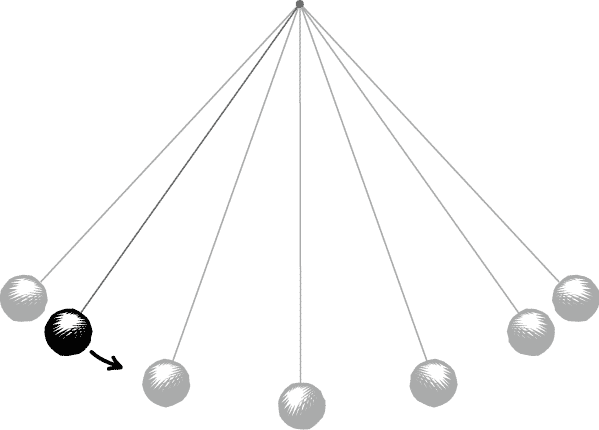
\includegraphics[width=0.8\linewidth]{Pictures/pendulum13}			
				\end{center}
			\end{column}	
			\begin{column}{.50\linewidth}
				\begin{center}
					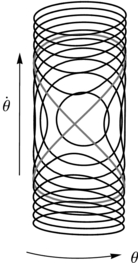
\includegraphics[width=0.45\linewidth]{Pictures/pendulum-phase-space}			
				\end{center}
			\end{column}	
		\end{columns}
		%
		\begin{defblock}[Symplectic Manifold]
			\includestandalone[width=0.95\textwidth]{Pictures/Figure_sym}	
		\end{defblock}
		%
		\begin{exblock}[$M = T^\ast Q$ is symplectic]
			$\omega = d \theta $ with
			$$ \left.\theta\right\vert_{(q,p)} (v) = p (\pi_\ast v) ~.$$
		\end{exblock}
	\end{column}
	\vrule{}
	\pause
	\begin{column}{.50\linewidth}
		\centering
		\textit{ "algebraic approach" to mechanics \dots}
		\vspace{1em}	
		\begin{defblock}[Classical Observables]
			Unital, associative, commutative algebra $C^\infty(M)$.
		\end{defblock}
		%
		\vspace{1em}
		\pause
		\begin{defblock}[Hamiltonian vector fields]
			$v_f \in \mathfrak{X}(M)$ such that:
			$$\iota_{v_f} \omega = -df \quad \text{(exact)}$$ %$\in B^1(M)$
			\small$v_f$ = \emph{Ham.v.f. pertaining to $f\in C^\infty(M)$}.
		\end{defblock}
		%
		\begin{defblock}[Poisson Algebra of Observables]
			$C^\infty(M)$ is a Poisson algebra with
			$$\{f,g\} = \iota_{v_g} \iota_{v_f} \omega = \omega(v_f,v_g) ~.$$
		\end{defblock}
	\end{column}
\end{columns}
\end{frame}
\note[itemize]{
	\footnotesize

	\item We work in the framework of multisymplectic geometry which is one of the possible generalizations of the well-established field of symplectic geometry.
	
	\item To recall what symplectic geometry is let me assume a particular point of view: mechanics.
	\\
	Idea:"
	Symplectic geometry is a branch of differential geometry studying symplectic manifolds; it originated as a formalization of the mathematical apparatus of classical mechanics and geometric optics."{\href{https://ncatlab.org/nlab/show/symplectic+geometry}{nlab}}
	
	Namely, a sym. mfd. is the geometric structure encoding the phase space of conservative, ordinary, classical, mechanical systems.
	
	\item $\theta$ = \emph{tautological 1-form}.
		$\theta$ evaluated at $p\in T^*Q$ in the fibre of $q\in Q$ and contracted with $v$ coincides with the form $p$ evaluated at $q$ and contracted with the push forward of $v$.
	
	\item We identify a special class of vector fields.
		Out of them one can define a Lie bracket.
	
	\item Poisson is a Lie algebra with the extra property of compatibility with the associative product (Leibniz rule)
}
%-------------------------------------------------------------------------------------------------------------------------------------------------

%-------------------------------------------------------------------------------------------------------------------------------------------------
\subsection{Multisymplectic geometry}

%-------------------------------------------------------------------------------------------------------------------------------------------------
\begin{frame}[fragile]{Multisymplectic manifolds} %Fragile -->workaround tikzcd
	\begin{defblock}[$n$-plectic manifold]
	\includestandalone[width=0.95\textwidth]{Pictures/Figure_multisym}	
	\end{defblock}
	%
	\begin{defblock}[Non-degenerate $(n+1)$-form]
		\begin{columns}
			\hfill
			\begin{column}{.5\linewidth}
				\centering{
				The $\flat$ (flat) bundle map is injective.
				}
			\end{column}
			\begin{column}{.5\linewidth}
				\[
				\begin{tikzcd}[column sep= small,row sep=0ex,
				/tikz/column 1/.append style={anchor=base east}]
				    \flat \colon T M \ar[r]& \Lambda^n T^\ast M \\
  						 v_x \ar[r, mapsto]& \iota_{v_x} \omega						
				\end{tikzcd}	
				\]
			\end{column}
		\end{columns}
	\end{defblock}
	%
	\pause
	\begin{defblock}[Hamiltonian $(n-1)$-forms]
		\begin{displaymath}
			\Omega^{n-1}_{ham} 	:=
			\biggr\{ H \in  \Omega^{n-1}(M) \; \biggr\vert \; 
				\exists X \in \mathfrak{X}(M) ~:~ d H = -\iota_X \omega \biggr\} 
			\end{displaymath}
	\end{defblock}
	%
	\pause					
	\begin{itemize}
		\item multisymplectic means \emph{going higher} in the degree of $\omega$\pause
		%\item 1-plectic $=$ symplectic
	\end{itemize}
	%
	\vfill
	%
	\begin{block}{Examples:}
		\begin{itemize}
			\item[$\bullet$] 1-plectic $=$ symplectic
			\item[$\bullet$] Any oriented $(n+1)$-dimensional manifold is $n$-plectic w.r.t. the volume form.
			\item[$\bullet$] The multicotangent bundle $\Lambda^n T^\ast Q$ is naturally $n$-plectic.
		\end{itemize}
	\end{block}			 
%
\end{frame}
\note[itemize]{
	\item Multisymplectic ($n$-plectic) geometry is a generalization of symplectic geometry in which the symplectic form is generalized from a closed $2$-form to a closed $n+1$-form, for $n\geq 1$.
	
	\item Historically, the interest in multisymplectic manifolds, has been motivated by the need of understanding the geometrical foundations of first-order classical field theories.
	\\ 
	The key point is that, just as one can associate a symplectic manifold to an ordinary classical mechanical system (e.g. a single
point-like particle constrained to some manifold), it is possible to associate a multisymplectic
manifold to any classical field system (e.g. a continuous medium like a filament or a fluid).
	
	\item We recognize the special class of forms, called Hamiltonian, determining the Hamiltonian vector fields.

	\item It is important to stress that mechanical systems are not the only source instances of this class of of structures. 
	For example, semisimple Lie groups
have a natural interpretation as 2-plectic manifolds.	

}
%---------------------------------------------------------------------------------------------------------------------------------------------------

%---------------------------------------------------------------------------------------------------------------------------------------------------
\subsection{Lie $\infty$-algebra of Observables}
\begin{frame}[fragile,t]{Lie $\infty$-algebra of Observables \emph{(Rogers)}}
	Consider $(M,\omega)$, $n$-plectic manifold,
	\begin{defblock}[$L-\infty$ Algebra of observables]
		Is a chain-complex\\
		\ifHandout
			\includestandalone{Pictures/Figure_Observables}	
		\else
			\includestandalone{Pictures/Frame_Observables}
		\fi
		
		\onslide<2->{with $n$ (skew-symmetric) multibrackets $(2 \leq k \leq n+1)$\\
			\includestandalone{Pictures/Equation_Multibracket}
		}
		%
	\end{defblock}

  \onslide<3->{
	\begin{itemize}
		\item \emph{higher analogue} of the \emph{Poisson algebra structure} associated to a symplectic manifold;
		\item Special instance of a more general object  called $L\-\infty$ Algebra.\\
		 (Generalization of Lie algebras. Jacobi identity is satisfied only up to a higher coherent chain homotopy.)
	\end{itemize}
	}
  \end{frame}
 \note[itemize]{

 	\item A Lie algebra is associated to an ordinary symplectic manifold (its Poisson algebra).
	(Underlying this is a Lie algebra, whose Lie bracket is the Poisson bracket.)
	Similarly, one associates an Lie-$n$ algebra to any $n$-plectic manifold.
 	% https://ncatlab.org/nlab/show/n-plectic+geometry 	 
 	 %https://ncatlab.org/nlab/show/Poisson+bracket+Lie+n-algebra
	 \item Basically, a Lie $n$-algebra is a chunk of the de Rham complex of $M$ with inverted grading and an extra structure called "multibrackets".
 	\item ( In the symplectic case it reduces to the corresponding Poisson algebra)
 	\item Rogers associated to any n-plectic mfd a $L\-\infty$ algebra, Zambon generalized it to the pre-n-plectic case.
 	\item Recognize in the definition of $[\cdot,\ldots,\cdot]_k$ the contraction with hamiltonian fields $v_\sigma$ w.r.t. $\sigma$.
  	\item Note $	\iota_{v_{\sigma_1}}\cdots\iota_{v_{\sigma_k}} = (-)^{(k-1)+(k-2)+\dots+1}\iota_{v_{\sigma_k}}\cdots\iota_{v_{\sigma_1}} = (-)^{\frac{k(k-1)}{2}}\iota_{v_{\sigma_k}}\cdots\iota_{v_{\sigma_1}}$ 
 	and the usual coefficient follows as $ (-)^{\frac{k(k-1)}{2}} = -\varsigma(k-1) = (-)^{k+1} \varsigma(k)$.
 }
%------------------------------------------------------------------------------------------------

%-------------------------------------------------------------------------------------------------------------------------------------------------
\subsection{(Homotopy) moment maps}
\begin{frame}{Moment maps}
	Consider a Lie algebra action $v:\mathfrak{g} \to \mathfrak{X}(M)$  preserving the $n$-plectic form $\omega$,
	\vfill
	\begin{columns}
		\begin{column}{.5\linewidth}	
	\textbf{Symplectic case $(n=1)$}
		\begin{defblock}[Comoment map pertaining to $v$]
			Lie algebra morphism
			$$ f: \mathfrak{g} \to C^\infty(M) $$
			such that
			$$ d~f (x) = -\iota_{v_x} \omega \qquad \forall x \in \mathfrak{g}~.$$
		\end{defblock}		
		\end{column}
		\begin{column}{.5\linewidth}	
	\textbf{Multi-symplectic case $(n\geq 1)$}
		\begin{defblock}[Homotopy comoment map \tiny (HCMM)]
			$L_\infty$-morphism 
			$$ (f_k) : \mathfrak{g} \to L_\infty (M,\omega)$$
			such that
			$$ d~f_1(x) = -\iota_{v_x} \omega \qquad \forall x \in \mathfrak{g}~.$$
		\end{defblock}		
		\end{column}
	\end{columns}	
	%
	\pause
	\centering \textbf{-- Conserved quantities --}
	%
	\begin{columns}
		\begin{column}{.5\linewidth}		
			\begin{propblock}[Noether Theorem]
				\small Fixed $H\in C^\infty_{\text{Ham}}(M)$ ($\mathfrak{g}$-invariant) ,
				$$\mathcal{L}_{v_H} f(x) = 0 \qquad \forall x \in \mathfrak{g}$$
			\end{propblock}
		\end{column}
		\begin{column}{.5\linewidth}			
			\begin{propblock}[RWZ16 Theorem]
				\small Fixed $H\in \Omega^{n-1}_{\text{Ham}}(M)$ ($\mathfrak{g}$-invariant),
				$$\mathcal{L}_{v_H} f_k(p) \in B^k(M) \qquad \forall p \in Z_k(\mathfrak{g})$$			
			\end{propblock}
		\end{column}
	\end{columns}



\end{frame}
\note[itemize]{
	\item  An infinitesimal symmetry is a lie algebra morphism such that $\mathcal{L}_{v_x} \omega = 0 ~ \forall x \in \mathfrak{g}$.
	\\ (It is also call an infinitesimal multisymplectic action and $v_x$ is the infinitesimal generator of the action, corresponding to $x \in \mathfrak g$.) 
	\item Essentially, admitting a comoment maps mean that $v$ acts via Hamiltonian vector fields.
	\item In mechanical terms, a moment map is a tool associated with a Hamiltonian action of a Lie group on a symplectic manifold, used to construct conserved quantities for the action.
	\item The name derives from the special case given by angular momentum in the dynamics of rigid bodies, 
	\item Notation [RWZ16]: H is called \emph{strictly invariant} and $f_k(p)$ are \emph{globally invariant}.
	\\
	$B^k(M)$ are exact differential k-forms and $Z_k(\mathfrak{g}$ are Eilenberg Chevalley homology k-cycles.
	
	\item Details about Reduction in frame \ref{frame:geometrysymmetries} of the  appendix.
	
}
%-------------------------------------------------------------------------------------------------------------------------------------------------





%-------------------------------------------------------------------------------------------------------------------------------------------------
\section{Work Done}
\checkpoint
%-------------------------------------------------------------------------------------------------------------------------------------------------
\subsection{Hydrodynamical homotopy moment map and Knots}
%-------------------------------------------------------------------------------------------------------------------------------------------------


%---------------------------------------------------------------------------------------------------------------------------------------------------
  \begin{frame}{Hydrodynamical $\mathfrak{g}$- action (joint work with M. Spera)}
	\begin{columns}[T] % align columns
	\begin{column}{.4\textwidth}
			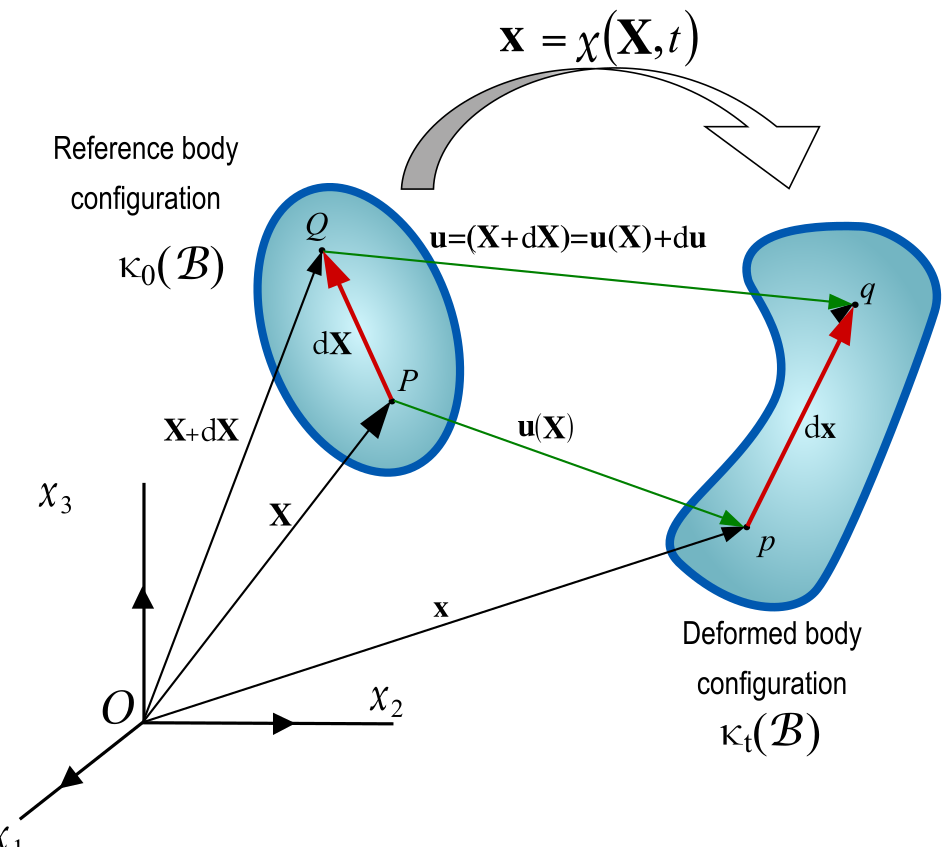
\includegraphics[width=\linewidth]{Pictures/Continuum_body_deformation}
	\end{column}
	%
	\hfill
	%
	\begin{column}{.6\textwidth}
		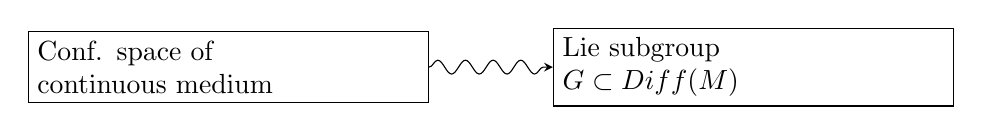
\begin{tikzpicture}[
			text width=0.4\linewidth,
			node distance=0.55\linewidth,
			]
			\node [rectangle,draw] (lhs) {Conf. space of\\ continuous medium};
			\node [rectangle,draw,right of=lhs] (rhs) {Lie subgroup \\$G \subset Diff(M)$};
			\draw[-stealth,decorate,decoration={snake}] (lhs) -- (rhs);
		\end{tikzpicture}

		Examples:
		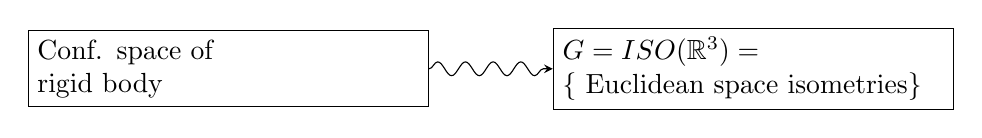
\begin{tikzpicture}[
			text width=0.4\linewidth,
			node distance=0.55\linewidth,
			]
			\node [rectangle,draw] (lhs) {Conf. space of\\ rigid body};
			\node [rectangle,draw,right of=lhs] (rhs) {$G=ISO(\mathbb{R}^3)=$\\ $\{$
				Euclidean space isometries$\}$};
			\draw[-stealth,decorate,decoration={snake}] (lhs) -- (rhs);
		\end{tikzpicture}
		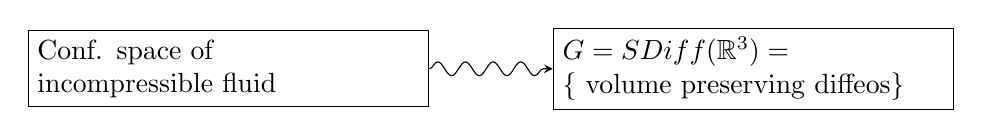
\begin{tikzpicture}[
			text width=0.4\linewidth,
			node distance=0.55\linewidth,
			]
			\node [rectangle,draw] (lhs) {Conf. space of\\ incompressible fluid};
			\node [rectangle,draw,right of=lhs] (rhs) {$G= SDiff(\mathbb{R}^3)=$\\ $\{$
				volume preserving diffeos$\}$};
			\draw[-stealth,decorate,decoration={snake}] (lhs) -- (rhs);
		\end{tikzpicture}
	\end{column}%
	\end{columns}
	\pause
  	\begin{lemblock}[$(\mathbb{R}^3,\nu = dx\wedge dy\wedge dz)$ is 2-plectic]
  		\begin{itemize}
  			\item \emph{(Easy proof)} $\quad \iota_v \nu = \frac{1}{2}\epsilon_{i j k} v^i dx^j \wedge dx^k = 0 \; \Leftrightarrow \; v=0 $;
  			\item \emph{(Conceptual proof)} $\quad \alpha^{(1)} = \ast \circ \flat$ is invertible.
  		\end{itemize}
  	\end{lemblock}
%		\begin{claimblock} Any oriented manifold is multisymplectic w.r.t. the volume form. \end{claimblock}

		\pause
		 	Consider a subalgebra of the infinitesimal action of $SDiff(\mathbb{R}^3)$:
		  	\begin{displaymath}
		  		\mathfrak{g} = sdiff_0(M) = \lbrace  X \in \mathfrak{X} \quad\vert\quad div X = 0, \textrm{\emph{ rapidly vanishing at }}\infty \rbrace
		  	\end{displaymath}
		  \alert{Does this $\infty$-dim. Lie algebra admit an HCMM?}	
		  	%\centering \alert{(Infinite dimensional Lie algebra!)}
  
  \end{frame}
  \note[itemize]{
	%\item  Now we are ready to get to the real business. Namely, give an explicitly construction of a HCMM related to hydrodynamics.
	\item We are working in the setting of \emph{geometric continuum mechanics} .\\
		Recall that the configuration space of a continuum object is encoded via diffeomorphisms. In the case of an incompressible fluid is encoded via volume-preserving diffeomorphisms.
	\item (Configution space is the set of spatial displacement of a mechanical systems. These are different from the \emph{physical states}.
	\item Such manifolds are infinite dimensional. Particular caution has to be taken in defining the smooth structure in this case.
	\item However, what really matters in the construction of a moment map is the infinitesimal action, i.e. the Lie algebra. In our case, the infinitesimal action to be considered is via divergence-free vector fields.
	\item (Notation): In the following M will be the 3 dimensional Euclidean Space.
	\item The simple but crucial observation is that the standard volume form on the euclidean space is a multisymplectic form.
	\item In the following, we will see that the standard Riemannian structure takes a role in our construction. 
	That was the reason to show also a "conceptual proof".
	\item Notation: $\ast = $ and $\sharp = $ are respectively the Hodge operator and the Riemannian sharp operator pertaining to the standard metric in $\mathbb{R}^3$.	
  }
%------------------------------------------------------------------------------------------------



%-------------------------------------------------------------------------------------------------------------------------------------------------
\begin{frame}[fragile]{Results (joint work with M. Spera)}
	\begin{itemize}[<+->]%[<alert@+>]
		\item Explicit construction of an HCMM for $SDiff_0 \circlearrowright (\mathbb{R}^3,\nu)$;
		\item Hydrodynamics interpretation: proved that this HCMM trasgresses to the standard hydrodynamical co-momentum map of  Arnol'd, Marsden and Weinstein and others;
		\item Generalized this construction to as special class of Riemannian manifolds (homological spheres);
		\item Proposed a covariant phase space interpretation of Brylinski's manifold of mildly singular links;
		% is exhibited upon resorting to the Euler equation for perfect fluids.
		\item Application to knot theory: reinterpretation of the (Massey) higher order linking numbers in terms of conserved quantities and determined the knot theoretic analogues of first integrals in involution.
		\item Aside: a semiclassical interpretation of the HOMFLYPT polynomial.% is also given, building on the Liu-Ricca hydrodynamical approach to the latter and on the Besana-S. symplectic approach to framing. 
	\end{itemize}
	%
	\pause
	\begin{center}
		\includegraphics{beamericonarticle} Appeared in \href{a}{arxiv:1805.01696} \includegraphics{beamericonarticle} \\ 
				\textbf{On some (multi)symplectic aspects of link invariants},\\
				\emph{AMM, Mauro Spera}. 			
	\end{center}	

\end{frame}
\note[itemize]{
	\item About the explicit construction see frame \ref{frame:explicithcmm} in appendix.
	\item About the hydrodynamical interpretation see frame \ref{frame:hydrointerpretation} 	%\item About the Riemmanian generalization see \ref{frame:riemannianhcmm}
	\item About the application to knots theory see frame \ref{frame:msknots1} and \ref{frame:msknots2} in appendix.
}
%-------------------------------------------------------------------------------------------------------------------------------------------------


%-------------------------------------------------------------------------------------------------------------------------------------------------
\subsection{Multisymplectic compact group actions on spheres}
%-------------------------------------------------------------------------------------------------------------------------------------------------

%-------------------------------------------------------------------------------------------------------------------------------------------------
\begin{frame}[fragile]{Cohomological obstruction to HCMM}
A HCMM is a sequence of linear maps:
			\begin{displaymath}
				(f)  = \big\lbrace f_k: \; \Lambda^k{\mathfrak g} \to L_{k-1} \subseteq \Omega^{n-k} 
				\;\big\vert\; 0\leq k \leq n+1  \big\rbrace
			\end{displaymath}
it can be interpreted as a primitive of a certain cocycle in the total complex of 
	\begin{displaymath}
		(C_\mathfrak{g}^{\bullet,\bullet} = \Lambda^{\geq 1} 
		\mathfrak{g}^*\otimes \Omega^\bullet(M), \delta_\text{CE},d),	
	\end{displaymath}
	%
	\pause
	\begin{propblock}[$\exists$ HCMM 
		$\Leftrightarrow ~ \lbrack\tilde{\omega}\rbrack=0\in H^{n+1}(C_\mathfrak g^\bullet,d_ {tot})$	
	]
		\begin{columns}
		\begin{column}{.5\textwidth}
			\begin{displaymath}
				\tilde{\omega} = \sum_{k=1}^{n+1} (-1)^{k-1} \iota^k_\mathfrak{g} \omega \in C_\mathfrak{g}^{n+1},
			\end{displaymath}		
		\end{column}
		\begin{column}{.5\textwidth}
			\begin{align*}
				\iota^k_\mathfrak{g} \colon \Omega^\bullet(M)
				&\to \Lambda^k \mathfrak{g}^\ast \otimes \Omega^{\bullet-k}(M)
				\\ \omega&\mapsto \omega_k = 
				\left(p \mapsto \iota_{v_p} \omega  \right) ,
			\end{align*}
		\end{column}		
		\end{columns} 
	\end{propblock}
	%
	\pause
	\begin{corblock}[Cohomological condition for $\vartheta:G\times M\to M$ compact Lie group action]
	$$\exists \text{ HCMM} 
		\Leftrightarrow ~[\vartheta^*\omega-\pi^*\omega]=0\in H^{n+1}(G\times M)$$ 
	\end{corblock}

\end{frame}
\note[itemize]{
	\item 
	The  corresponding total complex is given by
	\begin{displaymath}
		(C_\mathfrak{g}^{\bullet}, d_\text{tot} = 
		\delta_\text{CE}\otimes \text{id} + \text{id}\otimes d),
	\end{displaymath}
	where $d$ denotes the de Rham differential and $\delta_{CE}:\Lambda^k\mathfrak g^*\to \Lambda^{k+1}\mathfrak g^*$ the Lie algebra cohomology differential.
	According to the Koszul sign convention, $d_{\text{tot}}$ acts on an element of $\Lambda^k \mathfrak{g}^*\otimes \Omega^\bullet(M)$ as $\delta_\text{CE} + (-1)^k d$.

	\item PROP: the primitives of the natural cocycle $\tilde{\omega}$ are in one-to-one correspondence with comoments of $v$.
	
	\item COR: Let $\vartheta:G\times M\to M$ be a compact Lie group acting on a pre-multisymplectic manifold, preserving the pre-multisymplectic form $\omega$. 
A comoment exists if and only if $[\vartheta^*\omega-\pi^*\omega]=0\in H^{n+1}(G\times M)$.
	\item Note that here we employ the deRham cohomology of the product. This is different from the equivariant cohomology
	\item some more details in \ref{frame:cohomologicalproposition} of the appendix.
}
%-------------------------------------------------------------------------------------------------------------------------------------------------


%-------------------------------------------------------------------------------------------------------------------------------------------------
\begin{frame}[fragile]{Results (Joint work with L. Ryvkin)}
	Let $G\times M\to M$ be a compact Lie group preserving a pre-multisymplectic form $\omega$.
	\begin{itemize}
		\item Proved, without resorting on a specific model, that if $[\omega]\in H^\bullet(M)$ lies in the image of $q^*:H^\bullet_G(M)\to H^\bullet(M)$, then $\vartheta$ admits a comoment.
	\end{itemize}
	%\noindent\makebox[\linewidth]{\rule{\paperwidth}{0.4pt}}
	\pause
	\vspace{1em}
	Consider now $(M,\omega)$ to be a $n$-dimensional sphere together with the standard volume:
	%
			\begin{claimblock}
				Let $\vartheta:G\times S^n \to S^n$ be an effective,compact multisymplectic action,
				\begin{center}
					$\vartheta$ admits HCMM $~\Leftrightarrow~$ $n$ is even or $\vartheta$ is not transitive.
				\end{center}
			\end{claimblock}
	%
	\begin{itemize}
		\item 	Explicit construction for 
	$SO(n)~\circlearrowleft~S^{n}$ and
	$G_2~\circlearrowleft~(S^6,\phi)$
		\item  Explicit expression for the first 2 components of HCMM for 
			$SO(n+1)~\circlearrowleft~S^{n}$.
		 (Going higher can be set up as a computational problem. We sketched a prototype code in python.)
		 	\end{itemize}

	\pause
	\begin{center}
		\includegraphics{beamericonarticle} Appeared in \href{a}{arXiv:1906.08790} \includegraphics{beamericonarticle} \\ 
				\textbf{Multisymplectic actions of compact Lie groups on spheres},\\
				\emph{AMM, Leonid Ryvkin}. 			
	\end{center}	

\end{frame}
\note[itemize]{
	\item 	Let a compact Lie group $G$ act on a manifold $M$. Let $EG$ be a contractible space on which $G$ acts freely by $\vartheta^{EG}$. Then we define the equivariant cohomology of $M$ as $H^\bullet_G(M):=H^\bullet((M\times EG)/G)$, where $G$ acts on $M\times EG$ diagonally.

	\item As $EG$ might not be a manifold, we have to interpret $H^\bullet(\cdot)$ as a suituable cohomology theory (e.g. singular cohomology with real coefficients) in the above definition.
	
	\item As $G$ is compact, when $\vartheta:G\times M\to M$ is a free action, we have $H_G^\bullet(M)=H^\bullet_{dR}(M/G)$. For a not necessarily free action $\vartheta$, we still have the following diagram
	$$
		G\times (M\times EG) \xrightarrow{\vartheta\times \vartheta^{EG}}
		M\times EG \xrightarrow{q} (M\times EG)/G
	$$
	where $q$ is the projection to the orbits, which induces $q^*$ in cohomology.

	\item We gave	an intrinsic proof of Theorem which does not depend on the choice of a model for equivariant cohomology. 
	
	\item	
	Unlike the symplectic case, the converse statement does not hold in general. 
	Even if a (pre-)multisymplectic action of $G$ on $(M,\omega)$ admits a comoment, $[\omega]$ does not need to come from an equivariant cocycle. 
	
	\item 	
	First 2 component of HCMM for $SO(n+1)$ on $S^{n}$ (Going higher can be set up as a computational problem - we have a sketch of code in Python -, the first 2 component are easier due to the vanishing of the first two CE cohomology group of $G$)
}
%-------------------------------------------------------------------------------------------------------------------------------------------------



%-------------------------------------------------------------------------------------------------------------------------------------------------
\section{Work in Progress}
\checkpoint
%-------------------------------------------------------------------------------------------------------------------------------------------------
\subsection{Commutative diagram with gauge transformations and HCMM}

%-------------------------------------------------------------------------------------------------------------------------------------------------
\begin{frame}{Diagram for gauge transformations in symplectic geometry}
	%
	\vfill
	\includestandalone[width=\textwidth]{Pictures/Frame_BigDiagram_symplectic}
	%
	\begin{itemize}
		\item<2-> Given a Symp. mfd. $(M,\omega)$ there is a naturally associated Poisson algebra ...
		\item<3-> ... and also a Lie Algebroid.
		\item<4-> A Lie algebroid is a "controlled" $\infty$-dimensional Lie algebra;
		\item<5-> There is a natural embedding $C^\infty \to \Gamma(TM\oplus\mathbb{R})$;
		\item<6-> Consider a deformed structure $\tilde{\omega}= \omega + d B$ with $B\in C^\infty(M)$;
		\item<7-> There is a natural isomorphism in the Lie Alg.oids category,
		\item<8-> Considering $\mathfrak{g}\circlearrowleft M$ preserving $\omega$ and$\tilde{\omega}$ , \alert{the central square commutes!}.
	\end{itemize}
	%
\end{frame}
\note[itemize]{
	\item The horizontal embedding is  $f \mapsto (v_f,f)$;
	\item Vertical maps are also known as \emph{Gauge transformations}
}
%-------------------------------------------------------------------------------------------------------------------------------------------------

%-------------------------------------------------------------------------------------------------------------------------------------------------
\begin{frame}{Higher versions (WIP with M. Zambon)}
	Consider now $\omega$ multisymplectic...
	\vfill
	%
	\includestandalone[width=\textwidth]{Pictures/Frame_BigDiagram_k-plectic}
	%
	\vfill
	%
	\onslide<9->
	\textbf{TO DO:}
	\begin{itemize}
		\item[\CheckedBox] Diagram in the case $n=2$ (2-plectic manifolds and Courant algebroids)
		\item[\CheckedBox] Transgression to the diagram $n=2$ to a symplectic commutative diagram on loops.
		\item[$\square$] Explicit construction of $\mathbf{\color{red!60!black}\rightarrow}$ when $k\geq 3$. Commutativity? 
	\end{itemize}
\end{frame}
\note[itemize]{
	\item
}
%-------------------------------------------------------------------------------------------------------------------------------------------------


\subsection{Multisymplectic PDEs}

%-------------------------------------------------------------------------------------------------------------------------------------------------
\begin{frame}{Open questions on covariant observables (Preliminary)}
	%
	\begin{columns}
		%
		\begin{column}{.50\linewidth}
			\begin{center}
				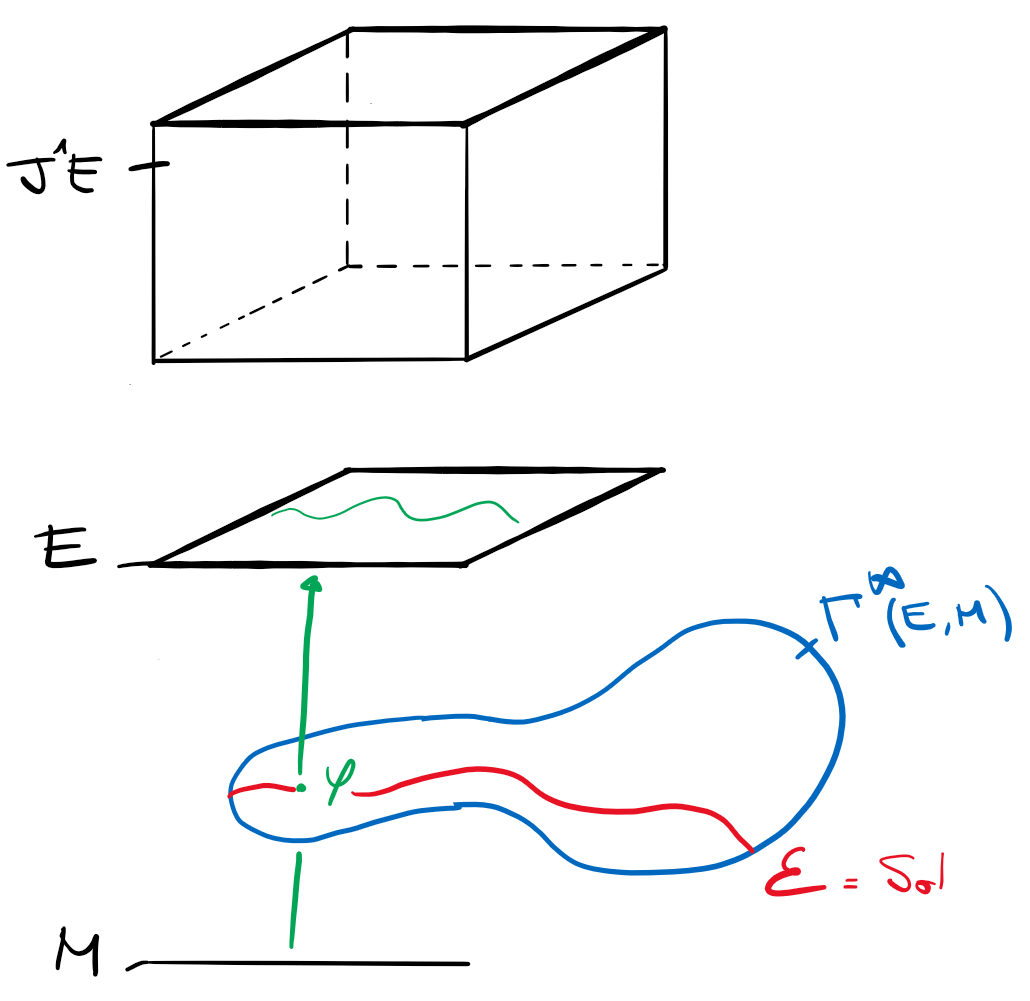
\includegraphics[width=0.9\linewidth]{Pictures/Covariant}			
			\end{center}
		\end{column}
		%
		\begin{column}{.50\linewidth}
			\begin{itemize}
				\item Consider a classical field $E\to M$ with I-order Lagrangian $\mathcal{L}$;
				\item<2-> $\mathcal{L}$ determines  
					\begin{itemize}
						\item[(a)] a multisymplectic structure on $J^1 E$,
						\item[(b)] a symplectic \emph{Diffiety} $(\mathcal{E})$ called \emph{Covariant phase space}\footnote{Suppose E-L operator being \emph{formally integrable}};
					\end{itemize}
				\item<3-> two different candidates for the role of \emph{physical observables}:
					\begin{itemize}
						\item[(a)] Lie infinity algebra $L_\infty (M,\omega)$;
						\item[(b)] Cochain complex $\bar{\Omega}^\bullet(\mathcal{E})$.
					\end{itemize}
				\item<4-> Questions:
					\begin{itemize}
						\item[-] What is their mutual relationship?
						\item[-] Application to \emph{Multisymplectic PDEs}?
						\item[-] Third actor: the \emph{Space of initial datas}.
					\end{itemize}																		
			\end{itemize}
		\end{column}
		%
	\end{columns}
\end{frame}
\note[itemize]{
	\item the two framework yields different candidates to the role of \emph{physical observable}:
	\item Note that in the classical ordinary case the space of initial data coincides with the phase space

}
%-------------------------------------------------------------------------------------------------------------------------------------------------


%------------------------------------------------------------------------------------------------
\section{Research plan}
\checkpoint
%------------------------------------------------------------------------------------------------
\begin{frame}{Research Plan}

\includestandalone[width=\textwidth]{timeline}


\color{green!80!black}
\begin{itemize}
	\item[\color{green!80!black}$\triangleright$] Sep 19 - Jan 20 :\color{black}
		\begin{itemize}
			\item[-] Finalize work on the commuting diagram with Marco Zambon,
			\item[-] Implement revisions to submitted papers.
		\end{itemize}
		\color{orange}
	\item[\color{orange}$\triangleright$] Jan 20 - Jul 20 :\color{black}
		\begin{itemize}%[label={-},noitemsep,topsep=0pt,parsep=0pt,partopsep=0pt]
			\item[-] Complete the manuscript of the thesis;
			\item[-] Develop a research proposal regarding multisymplectic PDEs;
			\item[-] Academic writing course.	
		\end{itemize}
		\color{red}
	\item[\color{red}$\triangleright$] Jul 20 - Oct 20 :\color{black}
		\begin{itemize}%[label={-},noitemsep,topsep=0pt,parsep=0pt,partopsep=0pt]
			\item[-] Submission of the PhD Thesis (by the end of July);
			%\item Report by the reviewers within 4 weeks;
			\item[-] Private defense at KU Leuven (around the end of September);
			\item[-] Public defense at UCSC Brescia	(by the end of October).
		\end{itemize}		
\end{itemize}

\end{frame}

%------------------------------------------------------------------------------------------------
\section{Joint PhD programme milestones}
\checkpoint
%------------------------------------------------------------------------------------------------

%------------------------------------------------------------------------------------------------
\begin{frame}[shrink]{Doctoral Training}
\begin{columns}
	\begin{column}{.50\linewidth}
	\begin{exampleblock}{	\textbf{\CheckedBox} Specific Skills (ECTS $\geq 4$)}
		\begin{itemize}%[label={-},noitemsep,topsep=0pt,parsep=0pt,partopsep=0pt]
			\item Topics in Symplectic and Multi-symplectic Geometry, 48h + exam, Brescia;
			\item Differential Topology and Geometry, 48h, Brescia;
			%\item Complex Geometry mod 1, 20h, Milano; 
			\item Introduction To Geometric Analysis: The Atiyah-Singer Index Theorem, 72h, Bilbao;
			\item Category Theory, 48h, Milano;
			\item Computational methods for the solution of Differential Equations, 12h + exam, Brescia;
			\item Classical and Quantum Knots, 20h, Milano-Bicocca;
			\item Summer School on Diffeology, Categories and Toposes, 24h, Izmir;
			%\item Summer School on Poisson Geometry, 24h, Toronto;
			%\item Symplectic and Poisson geometry, 18h, Bruxelles;
			%\item Introduction to Motivic Homotopy Theory, 24h, Verona;
			%\item XXII Summer Diffiety School, 24h, Bologna;
			%\item Summer School in Algebra and Topology, 24H, Lovain la Neuve
			\item \ldots		
		\end{itemize}
	\end{exampleblock}	
  \end{column}
  %
	\begin{column}{.50\linewidth}
	\begin{exampleblock}{	\textbf{\CheckedBox} Transferable Skills (ECTS $\geq 2$)}
		\begin{itemize}%[label={-},noitemsep,topsep=0pt,parsep=0pt,partopsep=0pt]
			\item Python for computational science, Cineca-Scai, $\sim 1$ ects;
			\item Control of biological functions mediated by nanostructured materials, Brescia, $\sim 0.25$ ects;
			\item Scientific computing with Python, Brescia, $\sim 0.75$ ects;
			\item Tools making research easy, Brescia, $\sim 0.1$ ects;
			\item \emph{(planned) Functional Programming and Domain-Specific Languages, Leuven, $\sim 0.75$ ects};
			\item \emph{(planned) Grant-writing workshop: Focus on FWO applications and beyond, Leuven, $\sim 0.5$ ects};
			\item \emph{(planned) Academic writing course, Leuven, $\sim 2$ ects}.
		\end{itemize}
	\end{exampleblock}	
  \end{column}
\end{columns}
\end{frame}
%------------------------------------------------------------------------------------------------

%------------------------------------------------------------------------------------------------
\begin{frame}[shrink]{Completed Tasks}

\begin{exampleblock}{\CheckedBox \textbf{Teaching activities $(\#\geq 10h)$}}
	\begin{itemize}%[label={-},noitemsep,topsep=0pt,parsep=0pt,partopsep=0pt]
		\item Exercise Class: Elements of Higher Geometry (15h), Brescia, A.Y. 17/18;
		\item Exercise Class: Differential Topology and Geometry (5h), Brescia, A.Y. 17/18;	
	\end{itemize}
\end{exampleblock}

\begin{exampleblock}{\CheckedBox \textbf{Active participation in conferences$(\#\geq 1)$}}
	\begin{itemize}%[label={-},noitemsep,topsep=0pt,parsep=0pt,partopsep=0pt]
		\item Poster at \emph{11th International Summer School on Geometry, Mechanics and Control}, Madrid , June 2017;
		\item Talk at \emph{12th International YOUNG RESEARCHERS WORKSHOP on Geometry, Mechanics and Control}, Coimbra, December 2018.
	\end{itemize}
\end{exampleblock}

\begin{exampleblock}{\CheckedBox \textbf{Seminars on the research topic $(\#\geq 2)$}}
	\begin{itemize}%[label={-},noitemsep,topsep=0pt,parsep=0pt,partopsep=0pt]
		\item \emph{Covariant Phase Space Via Multysimplectic Geometry}, Brescia, May 2017;
		\item \emph{On the Convenient Category of Diffeological Spaces}, Brescia, January 2018;
		\item \emph{On some (multi)symplectic aspects of link invariants}, Leuven, May 2018;
		\item \emph{(An introduction to )MultiSymplectic Geometry and Classical Field systems}, Leuven, February 2019;
		\item \emph{Multisymplectic Geometry and Knots}, Salerno, March 2019.
	\end{itemize}	
\end{exampleblock}	

\end{frame}
%------------------------------------------------------------------------------------------------

%------------------------------------------------------------------------------------------------
\begin{frame}{Pending Tasks}
	\begin{alertblock}{$\square$ \textbf{At least one Peer reviewed scientific paper}}
		\nocite{Miti2018,Miti2019}
		\bibliographystyle{unsrt}
		\bibliography{publications}
	\end{alertblock}

\end{frame}
%------------------------------------------------------------------------------------------------


  
%------------------------------------------------------------------------------------------------
% APPENDIX
%------------------------------------------------------------------------------------------------
\appendix
\section{EXTRA}
%\sectionpage
\begin{frame}
	\begin{center}
	\Huge\emph{Backup Slides}
	\end{center}
\end{frame}
\addtocounter{framenumber}{-1}

%------------------------------------------------------------------------------------------------
%- HandOut Flag -----------------------------------------------------------------------------------------
\newif\ifHandout
	\Handouttrue  %uncomment for the printable version

%- D0cum3nt ----------------------------------------------------------------------------------------------
\documentclass[beamer,10pt]{standalone}
	%\setbeameroption{show notes}
	




%- Packages ----------------------------------------------------------------------------------------------
%\usepackage{verbatim}
\usepackage[mode=buildnew,subpreambles=true]{standalone}
\usepackage{import}
\usepackage{amsmath, amssymb}
\usepackage{tikz}
%\usetikzlibrary{arrows,shapes,calc}
%\usetikzlibrary{shapes.callouts}
\usepackage{tikz-cd}
\usepackage{hyperref}
\usepackage[english]{babel}
\usepackage{stackengine}

%--Beamer Style-----------------------------------------------------------------------------------------------
\usetheme{toninus}



%--Beamer Style-----------------------------------------------------------------------------------------------
\usetheme{toninus}





%---------------------------------------------------------------------------------------------------------------------------------------------------
%- D0cum3nt ----------------------------------------------------------------------------------------------------------------------------------
\begin{document}
%------------------------------------------------------------------------------------------------

%##################################################################################
\section{Background Material}
%##################################################################################

%------------------------------------------------------------------------------------------------
\begin{frame}[fragile]{MS geometry and classical field mechanics}
		Consider a smooth manifold $Y$,
		\begin{columns}
			\hfill
			\begin{column}{.5\linewidth}
				\emph{Multicotangent bundle} $\bigwedge = \bigwedge^n T^\ast Y$\\
				is naturally $n$-plectic
			\end{column}
			\begin{column}{.4\linewidth}
				\[
				\begin{tikzcd}
					\Lambda \ar[d,"\pi"'] & T \Lambda \ar[d,"T \pi"] \ar[l] \\
					Y								& T Y \ar[l]
				\end{tikzcd}	
				\]
			\end{column}
		\end{columns}
	\pause
	\begin{defblock}[Tautological $n$-form]
		$\theta \in \Omega^n(\Lambda)$ such that:
		\begin{displaymath}
		\begin{split}
			\left[ \iota_{u_1 \wedge \ldots \wedge u_n} \theta \right]_\eta 
			&= \iota_{(T \pi)_\ast u_1 \wedge \ldots \wedge (T \pi)_\ast u_n} \eta \\
			&= \iota_{u_1 \wedge \ldots \wedge u_n} \pi^\ast \eta 
			\qquad \qquad \forall \eta \in \Lambda \, , \: \forall u_i \in T_\eta \Lambda 		
		\end{split}
		\end{displaymath}
	\end{defblock}
	\vfill
	\begin{columns}
		\begin{column}{.6\linewidth}
			\begin{defblock}[Tautological (multisymplectic) (n+1)-form]
				$$\omega := d \theta$$
			\end{defblock}
		\end{column}
		\begin{column}{.4\linewidth}
		 	\begin{claimblock}$\omega$ is not degenerate.\end{claimblock}	
		\end{column}
	\end{columns}	
	\pause
	\begin{keywordblock}
		\begin{tabular}{|c|c|c|}
			\hline 
			point-particles mechanics & $\rightsquigarrow$ & classical fields mechanics \\
			%(finite discrete DOF) & & (finite dimensional continuous DOF) \\
			\hline 
			symplectic & $\rightsquigarrow$ & multisymplectic \\ 
			\hline 
			Observables (Poisson) algebra & $\rightsquigarrow$ & Observables $L-\infty$ algebra
			 \\ 
			\hline 
			Co-moment map & $\rightsquigarrow$ & Homotopy co-momentum map \\ 
			\hline 
		\end{tabular} 
	\end{keywordblock}

	
\end{frame}
\note[itemize]{
	\item This example is significant from the perspective of geometric classical field theory:
		\begin{displaymath}
			\frac{\text{classical mechanics}}{\text{symplectic geo.}} =
			\frac{\text{classical field mechanics}}{\text{multisymplectic geo.}}
		\end{displaymath}
	\item Multicotangent bundle is the \emph{Higher analogue} of the cotangent bundle.
	(but it is not yet the analogue of a \emph{phase space}.)
\item The multiphase space is the sub-bundle of $n$-forms vanishing when contracted with 2 vertical fields.
  	\item The reason why this sub-bundle has a particular role is that it can be proved to be isomorphic to a suitable dual of the first Jet bundle.
  	\item For further details see Gotay et al. \href{https://arxiv.org/abs/physics/9801019}{arXiv:physics/9801019}. For a pictorial representation of all the structures involved in the geometric mechanics of I order classical field theories see appendix, pag: \ref{frame:Gimmsy}.
}
%------------------------------------------------------------------------------------------------	
	
%------------------------------------------------------------------------------------------------
\begin{frame}{Special classes of smooth objects} 
  	\begin{columns}
		\begin{column}[t]{.42\linewidth}		
			\begin{defblock}[Hamiltonian v.f.]
				$\mathfrak{X}_{ham} =  \left\lbrace X \in  \mathfrak{X} \right\vert \left. \iota_x \omega \textrm{ exact}  \right\rbrace$ 			
			\end{defblock}
			\begin{defblock}[Multisymplectic v.f.]
				$\mathfrak{X}_{ms} =  \left\lbrace X \in  \mathfrak{X} \right\vert \left. \mathcal{L}_X \omega = 0  \right\rbrace$ 	
			\end{defblock}
		\end{column}
		\begin{column}[t]{.58\linewidth}		
			\begin{defblock}[Hamiltonian $(n$-$1)-$forms]
				\begin{displaymath}
					\Omega^{n-1}_{ham} 	:=
					\biggr\{ H \in  \Omega^{n-1} \; \left\vert \; 
					\stackanchor{$\exists X \in \mathfrak{X}_{ham}$}{: $d H = -\iota_X \omega$} \right\} 
			\end{displaymath}
			\end{defblock}		
		\end{column}
  	\end{columns}
  	%
  	\vspace{0.5em}
  	%
  	\onslide<2->{
  	\begin{columns}
		\begin{column}[t]{.5\linewidth}	
			\centering\emph{Global symmetries}
			\begin{defblock}[Multisymplectic (Lie group) action]
				$\Phi: G \circlearrowright (M, \omega)$ \emph{right action} s.t. \\
				$$\hat{\Phi}(g)_\ast \omega = \omega \quad \forall g \in G$$
			\end{defblock}
		\end{column}
		\begin{column}[t]{.5\linewidth}			
			\centering\emph{Infinitesimal symmetries}
			\begin{defblock}[Multisymplectic (Lie algebra) action]
				$V: \mathfrak{g} \rightarrow \mathfrak{X} (M)$ \emph{Lie algebra morphism} s.t. \\
				$$\mathcal{L}_{V_\xi} \omega = 0 \quad \forall \xi \in \mathfrak{g}$$	
			\end{defblock}
		\end{column}
  	\end{columns}
  	}
  	%
  	\onslide<3->{		
	  	\begin{asideblock}[Hierarchy of conserved quantities]%Shades of...
	  		\begin{table}[] % http://tablesgenerator.com/
			\begin{tabular}{lllll}
					& strictly conserved & & & $\mathcal{L}_X \alpha= 0$ \\
				$\alpha \in \Omega^\bullet$ & globally conserved & along $X \in \mathfrak{X}$ & $\Leftrightarrow$ & $\mathcal{L}_X \alpha\in B $ (exact) \\
				  & locally conserved  & & & $\mathcal{L}_X \alpha\in Z $ (closed)                                
			\end{tabular}
			\end{table}
	  	\end{asideblock}
  	}
  	
  \end{frame}
  \note[itemize]{
  	\item Exactly as it happens in symplectic geometry, fixing a smooth form $\omega$ on $M$ yields a criterion for classifying vector fields and differential forms.
  	\\(Pay attention to the sign convention in defining the Hamiltonian vector fields)
  	\item Also, we can naturally select a special class of symmetries (global and infinitesimal) which preserve the fixed multisymplectic form.
  	\item Aside, we can start to see that, in this setting, measurable quantities are not only smooth functions but also differential forms with degree greater then zero.
  	For such objects can be defined weaker notions of conservation along a flow.
  	\item The idea to consider forms of various degree as observables do not fall out of the sky. 
  		For instance in a string there will be two kind of measurable quantities: extensive observable (1-forms), like the density, and intensive observables (0-forms), like the tension. 
 		%\href{https://en.wikipedia.org/wiki/Intensive_and_extensive_properties#Intensive_properties}{(wiki link on this terminology)}
  	\item Starting from this observation we can define the space of all possible observables (see next slide).
  }
%---------------------------------------------------------------------------------------------------------------------------------------------------


%------------------------------------------------------------------------------------------------
\begin{frame}[fragile,t]{Homotopy comoment map \emph{(Callies, Frégier, Rogers, Zambon)}}
  	%
		Consider a multisymplectic action $G \circlearrowright (M, \omega)$,
		%
		\begin{defblock}[Homotopy comoment map (HCMM)]				
			Is a sequence of linear maps:
			\begin{displaymath}
				(f)  = \big\lbrace f_k: \; \Lambda^k{\mathfrak g} \to L_{k-1} \subseteq \Omega^{n-k} 
				\;\big\vert\; 0\leq k \leq n+1  \big\rbrace
			\end{displaymath}
			%
			\includestandalone[width=0.95\textwidth]{Pictures/Frame_HCMM}			
			\emph{such that:}
			\begin{itemize}
				\item $f_0 = 0 $, $f_{n+1} = 0$ %(we have tacitly set $\Lambda^{-1}(M) = 0$)
				\item<2-> $-f_{k-1} (\partial p) = d f_k (p) + \varsigma(k) \alpha^{(k)} \quad \forall (k=1,\dots n+1), \; \forall p \in \Lambda^k(\mathfrak{g})$
			\end{itemize}
		\end{defblock}
		\begin{itemize}
			\item \emph{Higher analogue} of the ordinary comoment map $f\colon \mathfrak{g}\rightarrow C^\infty(M)$.
		\end{itemize}
  \end{frame}
  \note[itemize]{
		\item Notice that a HCMM pertains to an "infinitesimal" action of ${\mathfrak g}$ on $M$ 
			with ${\mathfrak g}$ being the Lie algebra of a generic Lie group $G$, 
			acting on $M$ by $\omega$-preserving vector fields.
		\item (Not.) $ p = \xi_1 \wedge \xi_2 \wedge \dots \wedge \xi_k$, 
			then $v_p = v_1 \wedge v_2 \wedge \dots \wedge v_k$ 
			where $v_i \equiv v_{\xi_i}$ are the fundamental vector fields associated to the action $G \circlearrowright M$.
	%	\item (Notation) $\iota(v_p) \omega = \iota(v_k)\dots\iota(v_1) \omega$
	%	\item $\varsigma(k) := - (-1)^{\frac{k(k+1)}{2}}$ 
		\item (Recall) $\alpha^{(k)}:= \iota(v_p) \omega = \iota(v_k)\dots\iota(v_1) \omega$
		\item $\partial \equiv \partial_k:  \Lambda^{k} {\mathfrak g} \to \Lambda^{k-1} {\mathfrak g}$  is the usual Eilenberg-Chevalley complex boundary operator (see appendix, pag: \ref{frame:CE-complex});
		\item The definition tells us that the {\it closed} forms
			$$\mu_k := f_{k-1} (\partial p) +  \varsigma(k) \iota(v_p) \omega 	$$
			must actually be {\it exact}, with potential $-f_k(p)$.  	
		\item The last equation tells us that an HCMM is not a chain complex morphism but is rather a chain complex homotopy between 0 and the multicontraction $\alpha$ (is a chain map by lemma 2.18 \cite{Ryvkin2016}).
		\item An HCMM is a L-$\infty$ morphism 
		$(f):\mathfrak(g)\rightarrow L(M)$ s.t. 
		$d f_1(\xi) = -\iota_{v_\xi} \omega$.\\
		\footnotesize{(Compare with the definition of ordinary comoment map: \\Lie algebra morphism 
		$J:\mathfrak(g)\rightarrow C^\infty(M)$ s.t. $ d J(\xi) =  -\iota_{v_\xi} \omega$)}
		
  }
%------------------------------------------------------------------------------------------------

%------------------------------------------------------------------------------------------------
\begin{frame}{Geometry of symmetries}\label{frame:geometrysymmetries}
	Basic mechanical structures are encoded in geometry. but there is another complementary geometrical property that's natural in physics: symmetry!
	\begin{alertblock}{Upshot}
		Continous symmetries are described by actions of a Lie group on $M$.
	\end{alertblock}
	\begin{block}{Noether}
		Presence of symmetries $\quad \Rightarrow \quad$ existence of conserved quantities.
	\end{block}	
	\begin{block}{Key concept:}
		Noether current are encoded in a \emph{moment map}  $\mu :M \rightarrow \mathfrak{g}^*$ (the dual of the comoment map $f$. 
	\end{block}
  \begin{columns}[T]
   	\begin{column}{.6\textwidth}
			\begin{block}{Symplectic reduction:}
			\begin{itemize}
				\item System dynamics should be restricted to level set of conserved observables in order to efficiently store dynamical properties.
				\item Under certain assumptions, $\mu^{-1}( 0 )/G$ is a symplectic manifold with an "induced" symplectic structure.
			\end{itemize}
			\end{block}
    \end{column}
    \begin{column}{.4\textwidth}	
			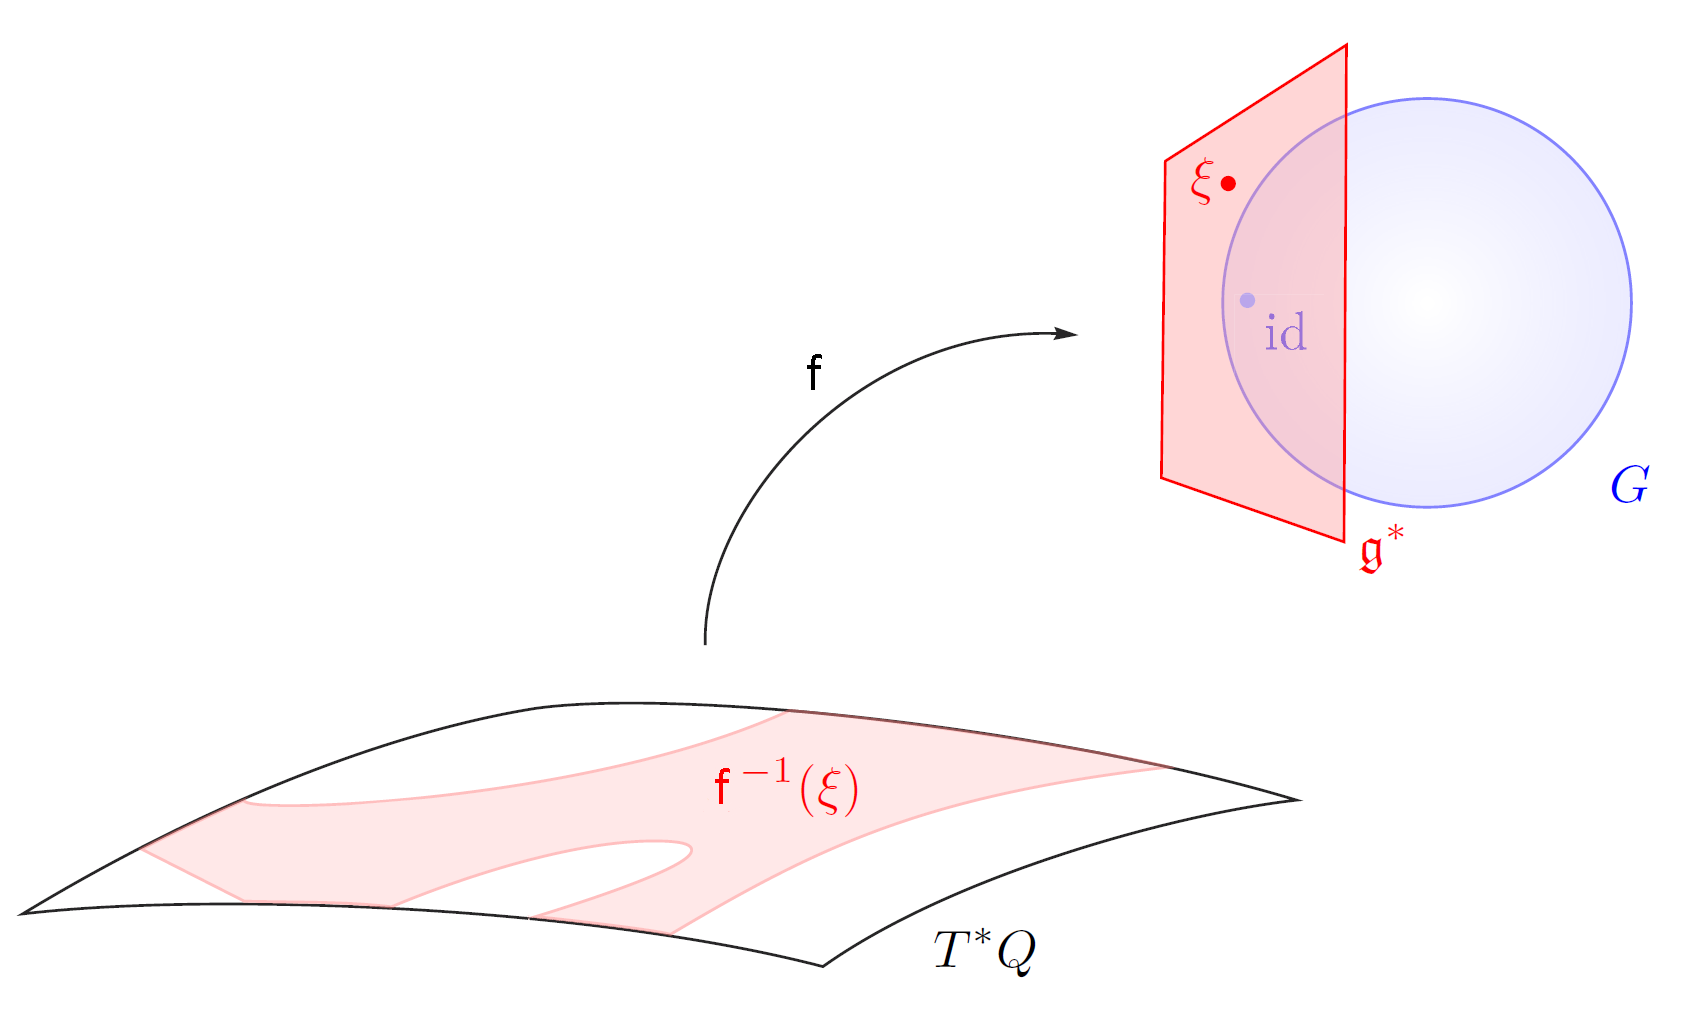
\includegraphics[width=\textwidth]{Pictures/Reduction} 
  	\end{column}
	\end{columns}			
\end{frame}
%------------------------------------------------------------------------------------------------

%##################################################################################
\section{Work Done with Mauro}
%##################################################################################

%------------------------------------------------------------------------------------------------
  \begin{frame}{Explicit Construction of the HCMM for $SDiff_0 \circlearrowright (\mathbb{R}^3,\nu)$}\label{frame:explicithcmm}
	\begin{columns}
		\begin{column}[c]{.5\linewidth}
		  	\begin{itemize}
		  		\item The observables are  $$L= \Omega^1_{\textrm{ham}}(\mathbb{R}^3)\oplus\Omega^0(\mathbb{R}^3)$$
		  		\item HCMM consists of a pair of functions:
					\begin{align*}
						f_1 &\colon \mathfrak{g} \rightarrow \Omega^1_{\textrm{ham}}(\mathbb{R}^3) \\
						f_2 &\colon \mathfrak{g}\wedge\mathfrak{g} \rightarrow C^\infty(\mathbb{R}^3)
					\end{align*}	
		  	\end{itemize}
		\end{column}	
	  	\hfill  	
		\begin{column}[c]{.5\linewidth}
  		\includestandalone[width=\textwidth]{Pictures/Figure_Euclid_Trigger}
 	 	\end{column}
 	 \end{columns}
 	\begin{columns}
		\begin{column}[c]{.8\linewidth}
		 	 \begin{itemize}
				\item Satisfying the following system:
					\begin{displaymath}
						\begin{cases}
							\textrm{d} f_1(\xi) = \iota_\xi \nu = -\alpha^1(\xi) \\
							\textrm{d} f_2(\xi_1 \wedge \xi_2) = f_1\left([\xi_1,\xi_2]\right) - \iota_{\xi_2}\iota_{\xi_1} \nu 
							 := \mu_2(\xi_1,\xi_2)\\
							f_2\left(\partial \xi_1 \wedge \xi_2 \wedge \xi_3 \right) = \iota_{\xi_3}\iota_{\xi_2}\iota_{\xi_1} \nu
						\end{cases}
					\end{displaymath}
				\item Results: 
					\begin{align*}
						f_1 &= \flat \circ {\rm curl}^{-1} \\
						f_2 &= {\rm grad}^{-1} \circ \sharp \circ \mu_2  
					\end{align*}	
		 	 \end{itemize}
 	 	\end{column}
		\begin{column}[c]{.2\linewidth}
 	 	\end{column}
 	 \end{columns}
  \end{frame}
	\note[itemize]{
		\tiny
		\item On the left there is the part of the Chevalley-Eilemberg complex that interact with the L-$\infty$ algebra of observables.
		\item On the right there is the whole de Rham complex of the manifold $M=\mathbb{R}^3$.
		\item Even if only $\Omega^1$ and $\Omega^0$ take part in the definition of a $HCMM$, the Riemmanian structure determine a correspondence with the rest of the de Rham complex.
		\item In order to give an HCMM for this action is necessary to give a solution of the system of 3 equations below.
		\item Recall: $ 	\ast: \Omega^k \rightarrow \Omega^{n-k}$ where $\ast \sigma$ is defined as the unique form such
		 that $ \omega \wedge \ast \sigma = \nu \lbrace \omega, \sigma \rbrace$ where 
		 $\langle,\rangle$ is the inner product on forms induced by the metric.
		\item Be aware of the sloppy notation: 
						the inverse of vector calculus differential operators are to be thought as their green operators.(There is no unique inverse of the curl!)
			Also, the second one, is the operation of taking a primitive $f_2={\rm d}^{-1} \circ \mu_2 $.
		\item UPSHOT: 
			\begin{itemize}
				\item We described a natural example motivated by physics,( momenta are related to vortices $\Leftarrow$).
				\item Transgression to loop spaces yields something already known in the context of fluid dynamics;		
				\item exemplified the generaf phenomenon that multisymplectic manifolds appear to be a \alert{"finite dimensional"} object able to encode features of \alert{"infinite dimensional"} mechanical systems.
			\end{itemize}
	}  
%---------------------------------------------------------------------------------------------------------------------------------------------------

%---------------------------------------------------------------------------------------------------------------------------------------------------
\begin{frame}[fragile]{Hydrodynamics interpretation}\label{frame:hydrointerpretation}
		Consider the loop spaces $L{\mathbb R}^3$,\\
		%
		\begin{propblock}[HCMM for $G\circlearrowright(\mathbb{R}^3,\nu)$ induces \\an ordinary co-mo.map for $G\circlearrowright (LS,\nu^{\ell})$]
			The HCMM $f \colon \mathfrak{g} \to L_{\infty}(\mathbb{R}^3,\nu)$ previously given
			\emph{transgresses}	 to
			\begin{displaymath}%\tag{Arnol'd-Marsden-Weinstein\\ hydrodynamical co-momentum map}
				\begin{tikzcd}[column sep= small,row sep=0ex]
					\lambda \colon& \mathfrak{g}	\arrow[r]& C^\infty(LS) \\
					& {\mathbf b}	\arrow[r, mapsto]
					& \displaystyle \biggr( \gamma \mapsto \lambda_b(\gamma) = - \oint_{\gamma} f_1({\mathbf b})  \biggr)	
				\end{tikzcd}	
			\end{displaymath}
			that is a  moment map for the induced action $G$ on the pre-symplectic loop space $(LM,\nu^{\ell})$. (Smooth space in the sense of Brylinski)
		\end{propblock}
		\begin{itemize}
			\item $\lambda$ corresponds to \emph{Arnol'd-Marsden-Weinstein hydrodynamical co-momentum map}  defined on $\infty$-dim. manifolds.
			\item<2-> $\Lambda = \left\lbrace \lambda_{\mathbf b} \right\rbrace_{{\mathbf b}\in\mathfrak{g}}$ is, up to sign, the {\it Rasetti-Regge current algebra}
			\item<3-> There is a naturally defined {\it Poisson brackets} on $\Lambda$:
				\begin{displaymath}
					\{ f_1({\mathbf b}), f_1({\mathbf c}) \} (\cdot):= \iota_{\mathbf c} \iota_{\mathbf b} \nu (\cdot)=
						\nu({\mathbf b}, {\mathbf c}, \cdot) = f_1([{\mathbf b},{\mathbf c}])
					-df_2 ({\mathbf b} \wedge {\mathbf c})
				\end{displaymath}
				\centering\footnotesize(Note: $\lambda$ is (infinitesimally) $G$-equivariant, i.e. $	\{\lambda_{\mathbf b}, \lambda_{\mathbf c} \} = \lambda_{[{\mathbf b}, {\mathbf c}]}$)
		\end{itemize}

    
\end{frame}
\note[itemize]{
  	\item[ ] \textbf{How all of this is relevant in Hydrodynamics?}
  	\item The loop space is the manifold, in the sense of Brylinsky, consisting of all smooth loops in ${\mathbb R}^3$.
  	\item Transgression can be seen as a pull-back along the evaluation map 
  		$${\rm ev}: L{\mathbb R}^3 \times {\mathbb R} \ni (\gamma, t) \mapsto \gamma(t) \in {\mathbb R}^3$$
  		  	For further details see appendix, pag: \ref{frame:LoopSpacesTransgression}.
  	\item Note that the (RR) current pertaining to ${\mathbf b} \in {\mathfrak g}$  is independent of the choice of $B$.
  			See appendix, pag: \ref{frame:RRcurrents} for other informations on this concept or \cite{Rasetti1975},\cite{Penna1992} for a deeper account.
  	\item In \cite{Callies2016} is proved a general result asserting that, roughly speaking,
			homotopy co-momentum maps transgress to homotopy co-momentum maps on loop (and even mapping) spaces. Further details in appendix, pag: \ref{frame:TransgressionHCMM}.
	\item Actually, the ansatz for $f_1$ term in the previous construction has been precisely motivated by this phenomenon. 
}
%------------------------------------------------------------------------------------------------

\begin{frame}{Hamiltonian forms related to a n-link}\label{frame:msknots1}

		
  	\onslide<1->{
  	\begin{columns}
		\begin{column}[c]{.7\linewidth}	
				Let $ L = \cup_{i=1}^n L_i$ be an oriented link in ${\mathbb R}^3$ 
				\\(components $L_i$, $i=1,\dots,n$ required to be  {\it trivial} knots)	
		\end{column}
		\begin{column}[c]{.25\linewidth}	
			\centering{
			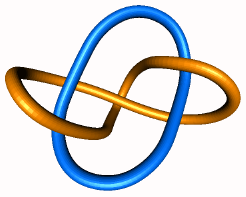
\includegraphics[width=0.75\linewidth]{Pictures/Whiteheadlink}
			}
		\end{column}
  	\end{columns}
  	}
		%
  	\onslide<2->{
  	\begin{columns}
		\begin{column}[t]{.5\linewidth}	
			\begin{defblock}[Vorticity 2-form]
				$$
				\omega_{L} := \sum_{i=1}^n \omega_{L_i}, \qquad d\omega_L = 0
				$$
				($\omega_{ L_i}$ = Poincar\'e dual associated to $L_i$)
			\end{defblock}
		\end{column}
		\begin{column}[t]{.5\linewidth}	
			\begin{defblock}[Velocity 1-form]
				$$
 					v_{ L} = \sum_{i=1}^n v_{L_i}, \qquad \qquad  dv_{L} = \omega_{ L}
				$$
				($v_{L_i} := \omega_{{\mathfrak a}_i}$ = Poincar\'e dual  of a disc ${\mathfrak a}_i$ 
				bounded by 	$L_i$ \footnotesize{(Seifert surface)}) 
			\end{defblock}						
		\end{column}
  	\end{columns}
  	}
  	%
  	\begin{columns}
		\begin{column}[t]{.3\linewidth}	
  		\onslide<2->{
  			\center
  			\vspace{-4ex}
				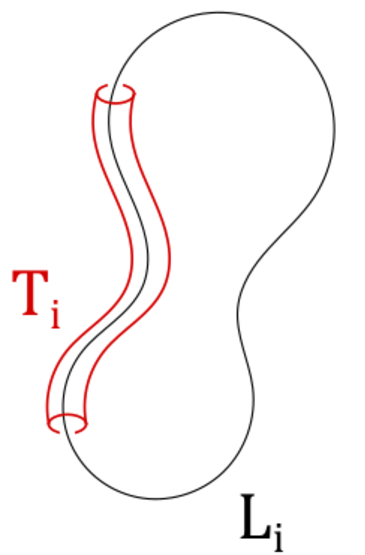
\includegraphics[width=0.6\linewidth]{Pictures/tubes}
	  	}			
		\end{column}
		\begin{column}[t]{.7\linewidth}	
  	\onslide<3->{
			\begin{propblock}[$v_{L}$ is a {\it Hamiltonian 1-form}]
				For each component $L_i$, the Hamiltonian vector field $\xi_{L_i}$ of 
				$v_{L_i}$ is $-\alpha^{-1}(\omega_{L_i})$.
				\\
				Explicitly, one has 
				\begin{displaymath}
					dv_L + \sum_{i=1}^n\iota_{\xi_{L_i}} \nu = 0 				
				\end{displaymath}
			\end{propblock}  	
  	}				
		\end{column}
  	\end{columns}
\end{frame}
\note[itemize]{
	\item $\omega_{ L_i}$ denote the Poincar\'e (or Thom) dual (class) associated to $L_i$: they are 2-forms localized in a 
 cross-section of a  suitable tubular neighbourhood $T_i$ around $L_i$ - with total fibre integral equal to one, or, as currents, 2-forms which are $\delta$-like on $L_i$
 
	\item $v_{L_i} := \omega_{{\mathfrak a}_i}$ is the Poincar\'e dual (class) of a disc ${\mathfrak a}_i$ bounding
$L_i$ (a Seifert surface for the trivial knot $L_i$). Precisely:
$$
\partial {\mathfrak a}_i = L_i, \qquad \qquad dv_{L_i} = d\omega_{{\mathfrak a}_i} = \omega_{L_i} = \omega_{\partial {\mathfrak a}_i},
$$
	\item
		Velocity 1-forms $v_i$ correspond (upon approximation of the associated Euler equation) to the so-called LIA (Linear Induction Approximation) or  {\it binormal evolution}
		of the ``vortex ring" $L_i$ (``orthogonal" to the discs ${\mathfrak a}_i$.
		
	\item Everything is up to choices of tubular neighbourhoods, Seifert surface and specific Poincar\'e dual.


}
%------------------------------------------------------------------------------------------------


%------------------------------------------------------------------------------------------------
\begin{frame}{Relation with Gauss linking number}\label{frame:msknots2}
		%
		\vspace{-2.5ex}
		%
  	\begin{columns}
		\begin{column}[t]{.5\linewidth}	
			\begin{defblock}[Chern-Simons 3-form]
				$$
					CS({L}) :=  v_{L} \wedge  \omega_{ L} 
				$$
			\end{defblock}
		\end{column}
		\begin{column}[t]{.5\linewidth}	
			\begin{defblock}[Helicity]
				$$
 					{\mathcal H}(L) = \int_{\mathbb{R}^3} CS({L})
				$$
			\end{defblock}						
		\end{column}
  	\end{columns}
	\pause
	\begin{propblock}[
		Choosing a parametrization $\mathbf{r}_i$ (in standard coordinates) for each $L_i$ 
		\begin{displaymath}
			{\mathcal H}(L)  = 
			\sum_{i,j=1}^n
			\,\frac{1}{4\pi}
			\oint_{\gamma_i}\oint_{\gamma_j}
			\frac{\mathbf{r}_i - \mathbf{r}_j}{|\mathbf{r}_i - \mathbf{r}_j|^3}
			\cdot (d\mathbf{r}_i \times d\mathbf{r}_j) =
			\sum_{i,j=1}^n \ell(i,j)
		\end{displaymath}
			$\bullet$ $\ell(i,j) = \ell(j,i)$ : Gauss linking number of components $L_i$ and $L_j$ if $i\neq j$\\
			$\bullet$ $\ell(j,j)$ : {\it framing} of $L_j$\\ 
			\phantom{-------}\footnotesize{ (i.e. $\ell(L_j, L_j^{\prime})$ with $L_j^{\prime}$ being a section of the normal bundle of $L_j$.)}\normalsize

		]
	\pause
  	\begin{columns}
		\begin{column}[c]{.7\linewidth}	
		\underline{Sketch}: Cosider a Hopf Link
			\begin{displaymath}
				L(C,C') = \eta_C \wedge \eta_{\Sigma'} + \eta_{C'} \wedge \eta_\Sigma =
				\eta_{P'} + \eta_{P}
			\end{displaymath}
		\end{column}
		\begin{column}[c]{.25\linewidth}	
			\centering{
			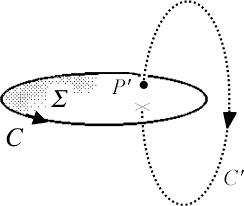
\includegraphics[width=0.75\linewidth]{Pictures/GaussLink}
			}
		\end{column}
  	\end{columns}
			Therefore $\int L(C,C') = \ell(C,C')$ 
			algebraically counts crossings of a component with a Seifert surface of a different one.			%sign is given by the orientation.
		\end{propblock}
		
\end{frame}
\note[itemize]{
	\item Our previous construction is heavily dependent on a lot of choices 
	but we end up with a quantity that only depends on the starting n-link.
	\item ${\mathcal H}(L)$ is invariant under ambient isotopies.\\
	However, non ambient isotopic links do not necessarily yield different linking numbers
	(it is not an universal invariant!).
  	\begin{columns}
		\begin{column}[c]{.5\linewidth}	
			\centering{
			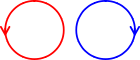
\includegraphics[width=0.5\linewidth]{Pictures/UnknotsGauss}
			}
		\end{column}
		\begin{column}[c]{.5\linewidth}	
			\centering{
			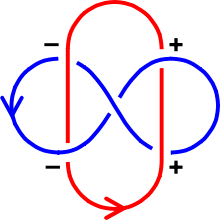
\includegraphics[width=0.35\linewidth]{Pictures/WhiteheadGauss}
			}
		\end{column}
  	\end{columns}	
	\item
		\begin{displaymath}
	\begin{split}
		\text{link}(\gamma_1,\gamma_2) &=\,\frac{1}{4\pi}
		\oint_{\gamma_1}\oint_{\gamma_2}
		\frac{\mathbf{r}_1 - \mathbf{r}_2}{|\mathbf{r}_1 - \mathbf{r}_2|^3}
		\cdot (d\mathbf{r}_1 \times d\mathbf{r}_2)\\[4pt]
		 &= \frac{1}{4\pi}\int_{S^1 \times S^1} \frac{\text{det}(\dot{\gamma_1}(s),
	 \dot{\gamma_2}(t),\gamma_1(s)-\gamma_2(t))}{|\gamma_1(s)-\gamma_2(t)|^3}\, ds \, dt
	\end{split}
	\end{displaymath}
}
%------------------------------------------------------------------------------------------------

%##################################################################################
\section{Work Done with Leonid}
%##################################################################################
%-------------------------------------------------------------------------------------------------------------------------------------------------
\begin{frame}[fragile]{Cohomological obstructions for compact groups}\label{frame:cohomologicalproposition}
	Let $\vartheta:G\times M\to M$ be a compact Lie group acting on a pre-multisymplectic manifold, preserving the pre-multisymplectic form $\omega$. 
	%
	\begin{propblock}
		[ $\exists$ (HCMM) $ 
			~\Leftrightarrow~ 
			\lbrack\vartheta^*\omega-\pi^*\omega\rbrack=0\in H^{n+1}(G\times M)$]
		Based on the sequence of isomorphisms:
		\begin{center}
			\begin{tikzcd}
	 			\Omega^\bullet(M,\vartheta) \ar[d,"\vartheta^\ast-\pi^\ast"] &\quad
				 & H_\text{dR}(M) \ar[d,"\vartheta^\ast-\pi^\ast"]  
				 & \lbrack \omega \rbrack \ar[d,mapsto]
				 \\ 
				 \Omega^\bullet(G\times M, r\times id) \ar["\cong",leftrightarrow]{d} &\quad
				 & H_\text{dR}(G\times M) \ar[leftrightarrow,"\cong"]{d}[swap]{\text{\tiny (K\"unneth)}} 
				 & \lbrack \vartheta^\ast \omega - \pi^\ast \omega \rbrack \ar[ddd,mapsto]
				 \\ 
				 \Omega^\bullet(G,r) \otimes \Omega^\bullet(M) \ar["\cong",leftrightarrow]{d}[swap]{} &\quad
				 & H_\text{dR}(G) \otimes  H_\text{dR}(M) \ar[d,"\cong",leftrightarrow]
				 \\ 
				 \Lambda^\bullet \mathfrak{g}^* \otimes \Omega^\bullet(M)\ar["\cong",leftrightarrow]{d} &\quad
				 & H_\text{CE}(\mathfrak{g}) \otimes  H_\text{dR}(M) 
				 \ar["\cong",leftrightarrow]{d} & 
				 \\
				 C_\mathfrak{g}^\bullet \oplus ( \mathbb{R}\otimes \Omega^\bullet(M))&\quad 
				 & H(C_\mathfrak{g}^\bullet)\oplus H_\text{dR}(M)
				 & \lbrack \tilde{\omega}\rbrack
			\end{tikzcd}
		\end{center}						
	\end{propblock}
\end{frame}
%-------------------------------------------------------------------------------------------------------------------------------------------------


%------------------------------------------------------------------------------------------------
\end{document}
%------------------------------------------------------------------------------------------------

%------------------------------------------------------------------------------------------------
\begin{frame}[t]{Other aknowledgements}
	\begin{itemize}
		\item Picture - Pendulum 13
			\url{https://andrewjobling.com.au/home-1/everything-okay-becasue-pendulum-swings/}
		\item Picture - Pendulum Phase Space
			\url{https://iopscience.iop.org/article/10.1088/0143-0807/33/2/231}
				\item Picture - Continuum deformation
			\url{https://commons.wikimedia.org/wiki/File:Displacement_of_a_continuum.svg}
		\item Animation - Reidmester moves
			\url{http://realworldmath.tumblr.com/post/57577812688/what-the-hell-is-knot-theory-knot-theory-is-one}
		\item Animation - Bubble rings
			\url{https://www.facebook.com/Nassim.Haramein.official/videos/596203997519126/}
		\item Picture - Whithead link 
			\url{https://en.wikipedia.org/wiki/Whitehead_link}
		\item Picture - Gauss linking number 
			\url{https://www.maths.ed.ac.uk/~v1ranick/papers/ricca.pdf}
		\item Picture - Borromean Rings
			\url{https://en.wikipedia.org/wiki/Borromean_rings}	
	\end{itemize}
\end{frame}
%------------------------------------------------------------------------------------------------


%------------------------------------------------------------------------------------------------
\end{document}

